\documentclass[xcolor=pdftex,dvipsnames,table]{beamer}

\mode<presentation>
{
  \usetheme{Singapore}
  \usecolortheme{seahorse}
  \setbeamercovered{dynamic} %invisible
}

\usepackage[utf8]{inputenc}
\usepackage[english]{babel}
\usepackage{minted}

\graphicspath{ {./images/} }

%%%%%%%%%%%%%%%%%%%%%%%%%%%%%%

\title{Effect Handlers in Scope}
% \subtitle{}
\author[Wu, Schrijvers, Hinze]
{N.~Wu\inst{1} \and T.~Schrijvers\inst{2} \and R.~Hinze\inst{1}}

\institute[VFU] % (optional)
{
  \inst{1}%
  University of Oxford
  \and
  \inst{2}%
  Ghent University
}

\date[ICFP 2014]{ICFP 2014}

% \logo{
\includegraphics[height=0.5cm]{haskell-logo.png}}

%%%%%%%%%%%%%%%%%%%%%%%%%%%%%%

\AtBeginSection[]
{
  \begin{frame}<beamer>
      \frametitle{Table of Contents}
      \tableofcontents[currentsection]
  \end{frame}
}

\begin{document}

\defverbatim[colored]\mycode{%
  \begin{minted}[fontsize=\footnotesize]{haskell}
data Backtr a
  = BReturn a -- Success
  | BFail -- Failure
  | Backtr a :<> Backtr a -- Choice
  deriving (Read, Show, Functor)

instance Functor Backtr => Applicative Backtr where
  pure = BReturn
  (<*>) = ap

instance Applicative Backtr => Monad Backtr where
  return :: a -> Backtr a
  return = pure

  (>>=) :: Backtr a -> (a -> Backtr b) -> Backtr b
  BReturn a >>= r = r a
  BFail >>= _ = BFail
  (p :<> q) >>= r = (p >>= r) :<> (q >>= r)
  \end{minted}                      
}

\frame{\titlepage}

\section{Test section one}
\begin{frame}
  \frametitle{Foo}
  % {\color{Red!100} A B C}
  %
  \begin{columns}[c]
    \column{1.5in}
    This is a line\\ \pause
    This is a line

    \column{1.5in}
    \framebox{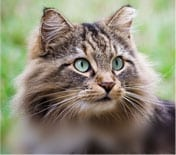
\includegraphics[width=1.5in]{cat.jpg}}
  \end{columns}
\end{frame}

\section{Test section two}

% \begin{frame}\frametitle{Tic-Tac-Toe via {\tt tabular}}\setbeamercovered{invisible}{\Huge\begin{center}\begin{tabular}{c|c|c}\onslide<9->{O}  & \onslide<8->{X} & \onslide<2->{X} \\ \hline\onslide<6->{X}  & \onslide<3->{O} & \onslide<5->{O} \\ \hline\onslide<10->{X} & \onslide<7->{O} & \onslide<4->{X}\end{tabular}\end{center}}\end{frame}

\begin{frame}[t] % vertical flushing
  \frametitle{Third slide}
  \framesubtitle{This is a subtitle}
  \begin{theorem}
    This is a theorem
  \end{theorem}
  \begin{proof}
    Very interesting proof
  \end{proof}
\end{frame}

\begin{frame}{Title}
  \begin{block}{Question}
    How many cats ?
  \end{block}
  \begin{block}{Answer}
    Two
  \end{block}
  \begin{block}{enum me}
    \begin{enumerate}
        \item<1-> This is a
        \item<2-> theorem
    \end{enumerate}
  \end{block}
\end{frame}

\section{Third section}

\begin{frame}{Title}
  \begin{block}{Question}
    Is every even number the sum of two primes?
    \cite{Goldbach1742}
  \end{block}
\end{frame}

\begin{frame}[fragile]
  \frametitle{An algorithm for finding prime numbers.}
  \mycode
\end{frame}

%%%%%%%%%%%%%%%%%%%

\begin{thebibliography}{5}
  \bibitem{Goldbach1742}[Goldbach, 1742]
  Christian Goldbach.
  \newblock A problem we should try to solve
\end{thebibliography}

%%%%%%%%%%%%%%%%%%%%%

\end{document}

